\documentclass[PICOReport.tex]{subfiles}

\begin{document}

%To cover: Galaxy Formation, Clusters, Reionization, point sources (probably moves to a new section called 'Legacy Science')

{\bf Physics of Reionization}

The reionization of the Universe imprints multiple signals in the CMB, in both temperature and polarization.  In polarization, the most important reionization signal is the large-scale $E$-mode power sourced by the scattering of the temperature quadrupole during this epoch.  This signal allows a direct measurement of the optical depth, $tau$, with very little degeneracy with other parameters (and, to some extent, a measurement of the reionization history itself).  In contrast, inference of $\tau$ from the $TT$ power spectrum is hindered by its direct degeneracy with the scalar fluctuation amplitude.  Thus, large-scale $EE$ power spectrum measurements are a unique and crucial observable to constrain this parameter.  If measurements of $\tau$ are not improved beyond the current uncertainties from {\em Planck}, inference of several new aspects of cosmological physics (e.g., neutrino mass) will be severely hindered.  PICO is the ideal experiment to make this measurement.  Its noise level and frequency coverage permit a cosmic-variance-limited constraint on $\tau$, i.e., $\sigma(\tau) \approx 0.002$.  We verify this expectation via an explicit forecast following the methodology described in~\citet{errard_feeney_2015}, assuming PICO measurements of the $TT$, $TE$, $EE$, $BB$, and $\phi\phi$ power spectra, with the latter inferred via the iterative $EB$ estimator.  The polarized dust and synchrotron levels match those measured by {\em Planck}~\citep{PlanckFG2015}, including spatial variations, and are cleaned using a parametric maximum-likelihood approach.  Fitting a $\Lambda$CDM$+r$ model, for both the PICO ``requirements'' and ``CBE'' configurations, we find $\sigma(\tau) = 0.002$.  With the exquisite control of systematics needed for the much smaller primordial $BB$ signal, these are not a concern for $EE$ (and hence $\tau$).

In temperature, the most important small-scale imprint is that sourced by the ``patchy'' kinematic Sunyaev-Zel'dovich (kSZ) effect, due to the peculiar velocities of free electron bubbles around ionizing sources (e.g., galaxies or quasars).  The total kSZ power spectrum receives contributions from both the patchy reionization signal and ``late-time'' sources, e.g., the intergalactic and intracluster media.  The reionization and late-time signals are expected to have comparable amplitudes~\citep{Shaw2012,MMS2012,Battaglia2013}.  With constraints on the late-time contribution from other information (e.g., cross-correlations), effective small-scale foreground removal, and with the primary CMB $TT$ power spectrum constrained by inference from the $EE$ power spectrum, it is possible to extract reionization constraints from the small-scale kSZ power spectrum~\citep{calabrese/etal/2014}.

Fig.~\ref{fig:ReionizationPICO} presents forecasts for reionization constraints obtained from PICO's measurement of $\tau$ in combination with ground-based Stage-III (CMB-S3) constraints on the kSZ power spectrum (note that PICO will also provide some large-scale information on the kSZ power spectrum).  Constraints from existing Planck data and observations at other wavelengths are also presented.  The PICO measurement of $\tau$ is essential for breaking degeneracies and allowing simultaneous precise constraints to be placed on both the mean redshift and duration of reionization.

\begin{figure}
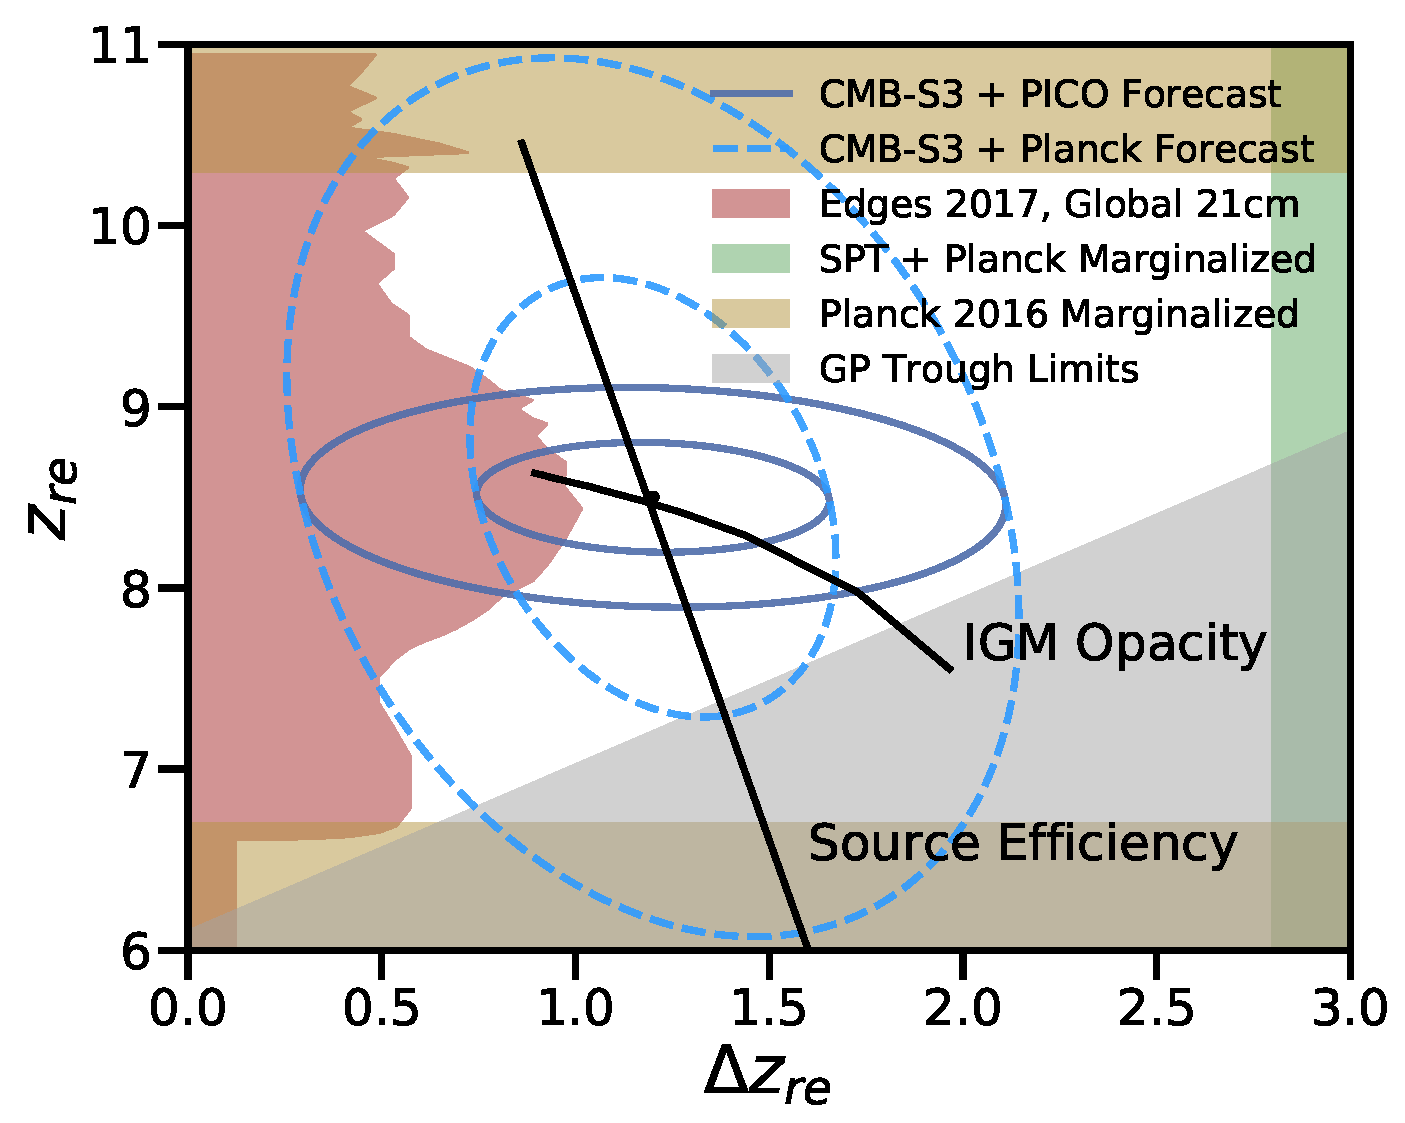
\includegraphics[width=0.8\textwidth]{images/Reionization_Contours_zbar_delz_PICO_NEW.pdf}
\caption{\label{fig:ReionizationPICO} Summary of constraints on the mean redshift and duration of reionization. The forecasts show 68\% and 95\% confidence-level contours for PICO combined with CMB-S3 experiments and Planck combined with CMB-S3 experiments (dark blue and dashed blue, respectively). The solid black lines illustrate how the IGM opacity and source efficiency model parameters map onto this parameter space. The forecasted PICO constraints are compared to: current exclusion limits for the mean redshift of reionization from Planck, shown by the yellow bands \citealp{planck2018:parameters}; recent exclusion limits from the global 21 cm signal measured by EDGES, shown with the red band \citealp{edges2017}; exclusion limits from measurements of the Gunn-Peterson trough from fully absorbed Lyman$\alpha$ in quasar spectra, shown by the grey band \citealp{Fan2006}; exclusion limit on the duration of reionization from Planck and SPT data, shown by the green band \citealp{planck_reio:2016}.}
\end{figure}

In addition to these signals, reionization also leaves specific non-Gaussian signatures in the CMB.  In particular, patchy reionization induces non-trivial 4-point functions in both temperature~\citep{SmithFerraro2017} and polarization~\citep{DvorkinSmith2008}.  The temperature 4-point function can be used to separate reionization and late-time kSZ contributions.  Combinations of temperature and polarization data can be used to build quadratic estimators for reconstruction of the patchy $\tau$ field, analogous to CMB lensing reconstruction.  \textbf{Are we planning to try to forecast these here?}

\textbf{FIGURE: $\tau$ constraint, kSZ power spectrum constraints, perhaps patchy $\tau$ reconstruction constraints? I assume the four-point estimator does not look promising given the relatively low resolution of PICO, but we can check the Smith papers.  This will essentially be an analog of Fig. 39 of the SO forecasting paper (Nick and Marcelo have the relevant code).}


The Sections below need to be rearranged to match other Science Objective(s) from the STM, but to also relay the 
breadth of science reachable by PICO, even if those goals are not in the STM. 

{\bf Structure Formation via Gravitational Lensing}


Measurements of the CMB reveal structure imprinted not only at the early time of recombination, but also at nearly every significant ensuing epoch in cosmic history.  In particular the matter between us and the CMB last-scattering surface will deflect the path of CMB photons, a process known as gravitational lensing.  Although the lensing of the CMB is a weak signal, targeted statistical estimators enable its  extraction.  
The detection of the lensing signal has rapidly progressed, from the first detections in 2007-8 \citep{2007PhRvD..76d3510S, 2008PhRvD..78d3520H} to the recent $ 40\sigma$ measurement by the {\it Planck} team \cite{2018arXiv180706210P}.  When applied to a rich dataset such as that expected from the PICO satellite, these estimators will provide a map of all the matter in the Universe in projection, with the most sensitivity at redshift $z \simeq 2$ and down to scales of approximately ten arcminutes.  

Forecasts show that the power spectrum of lensing in this map can be detected at approximately 580$\sigma$ or 650$\sigma$ for the requirement or CBE configurations, respectively.  Such high signal to noise measurements represent an order of magnitude improvement over the current state of the art, obtained by the  {\it Planck} team.  Figure \ref{fig:lensingNoisePICO} shows noise curves from the reconstruction of CMB lensing.  

\begin{figure}
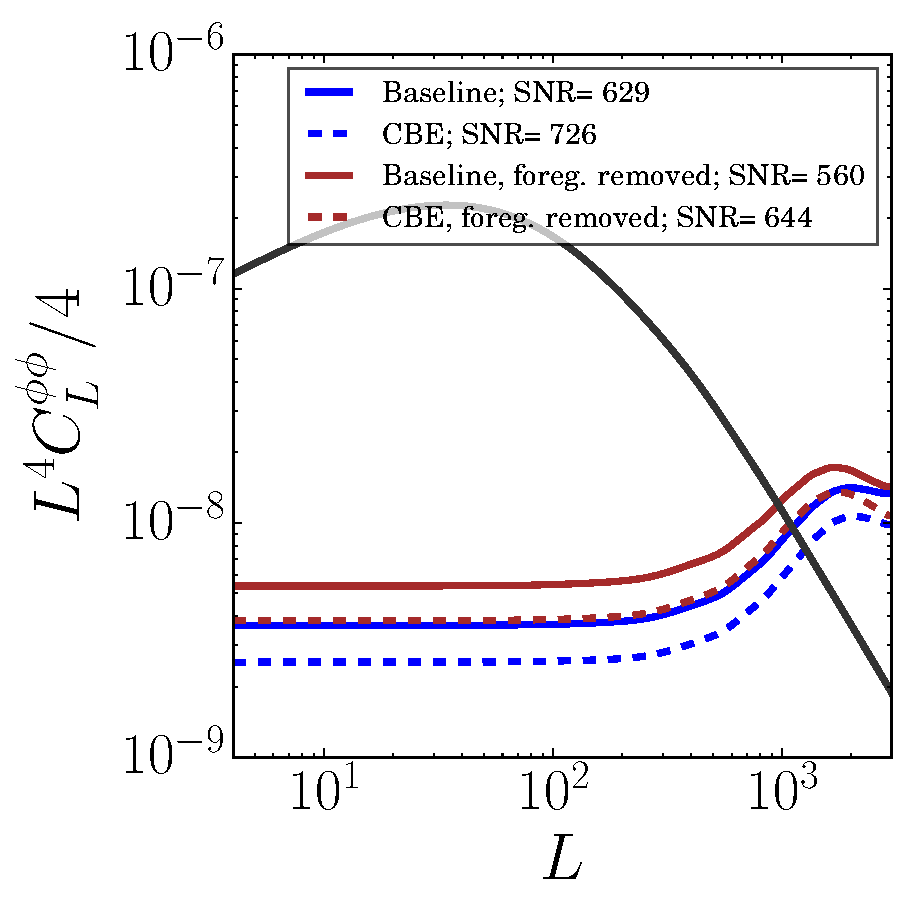
\includegraphics[width=0.8\textwidth]{images/lensingNoisePICO.pdf}
\caption{\label{fig:lensingNoisePICO} Lensing noise curves for various experimental configuraitons, showing the noise per mode of the reconstructed lensing field.  The  signal curve, the CMB lensing power spectrum is shown in grey; mapping of dark matter is possible at modes  where the noise curves fall below this signal.  Shown in solid are the performance of the $EB$ polarization estimator, including iterated delensing; this estimator performs best on large angular scales.  On smaller angular scales the temperature ($TT$) estimator shows the best performance. The associated signal to noise ratio for the lensing power spectrum is 570 for the 'requirement' configuration and 650 for the 'CBE'  configuration.}
\end{figure}


Lensing breaks the highly symmetric configuration of  primordial density fluctuations appearing as $E$ modes on the sky, turning some of these into $B$ modes.  If not accounted for, this effect yields an  noise floor on the large-scale $B$ modes that can be measured from the early Universe.  However, maps of $E$ modes and of the lensing field, both of which will be obtained with PICO data, can be used together to create a template for these lensed $B$ modes.  This template can then be subtracted from the measured $B$ modes to obtain improved performance, in a process known as ``delensing'' \citep{2004PhRvD..69d3005S,2012JCAP...06..014S}.  Forecasts show that up to 80\% of the lens-induced $B$ mode power can be removed in the 'requirement' configuration, with this number becoming 85\% for the current best estimate.  



\begin{itemize}
\item Delensing and neutrino mass constraints assumed to go in fundamental physics chapter
\item Cross-correlations: what to focus on here?
\item CMB halo lensing: cluster mass calibration
\end{itemize}

{\bf Physics of Galaxy Formation via the Sunyaev-Zel'dovich (SZ) Effects}

Not all CMB photons propagate through the universe freely, about 6\% of them are Thomson-scattered by free electrons in the intergalactic medium (IGM) and intracluster medium (ICM). These scattering events leave a measurable imprint on CMB temperature fluctuations called secondary anisotropies, and they contain a wealth of information from how structure grows to the thermodynamic history of baryons. A fraction of these photons produce Sunyaev--Zel'dovich effects~\citep{SZ1969,SZ1972}. The thermal SZ effect (tSZ) is the increase in energy of CMB photons due to scattering off hot electrons. This results in a spectral distortion
%, proportinal to the electron pressure,
 of the CMB blackbody that corresponds to a decrement in CMB temperature at frequencies below 217 GHz and an increment at frequencies above. The kSZ is the Doppler shift of CMB photons Thomson-scattering off free electrons that have a non-zero peculiar velocity with respect to the CMB rest frame. 
%This produces small shifts in the CMB temperature proportional to the radial velocity of the object and its optical depth.
The amplitdue of tSZ and kSZ proportional to the integrated electron pressure (tSZ) and momentum (kSZ) along the line of sight, thus contain information about the thermodynamic properties of the IGM and ICM 
%since their magnitudes are proportional to the integrated electron pressure (tSZ) and momentum (kSZ) along the line of sight.
The tSZ effect can be used to esemble statisitcs of galaxy clusters, which contain cosmological information as well as provide uniform cluster samples for galaxy formation studies in dense enviroments.
%
%\item Cosmological parameters from the abundance of tSZ-detected clusters and statistics of component-separated tSZ maps.
%\item Thermodynamic properties of galaxies, groups, and clusters from combined tSZ and kSZ cross-correlation measurements.
%\item Measurements of peculiar velocities, which are powerful cosmological probes on large scales, through the kSZ effect.
%\item Patchy reionization which imprints the CMB through higher order moments of the kSZ effect.

{\bf Galaxy Clusters}

%Through the tSZ PICO will produce a large all sky catalog of 

Galaxy clusters found via the tSZ provides a well defined sample with a simple to model selection function. Sample of clusters such as these are easy to use for cosmological inferences and studies of galaxy evolution in dense environments. 
Points to still hit.
High z sample,
Numbers,
most massive cluster all over the whole sky,
Cosmology.

\begin{itemize}
\item{Thermal SZ Effect}
\begin{itemize}
\item Cluster count forecast
\item{$y$-map and tSZ auto-power spectrum: figure with signal and NILC noise curve(s) [M. Remazeilles]}

\begin{figure}
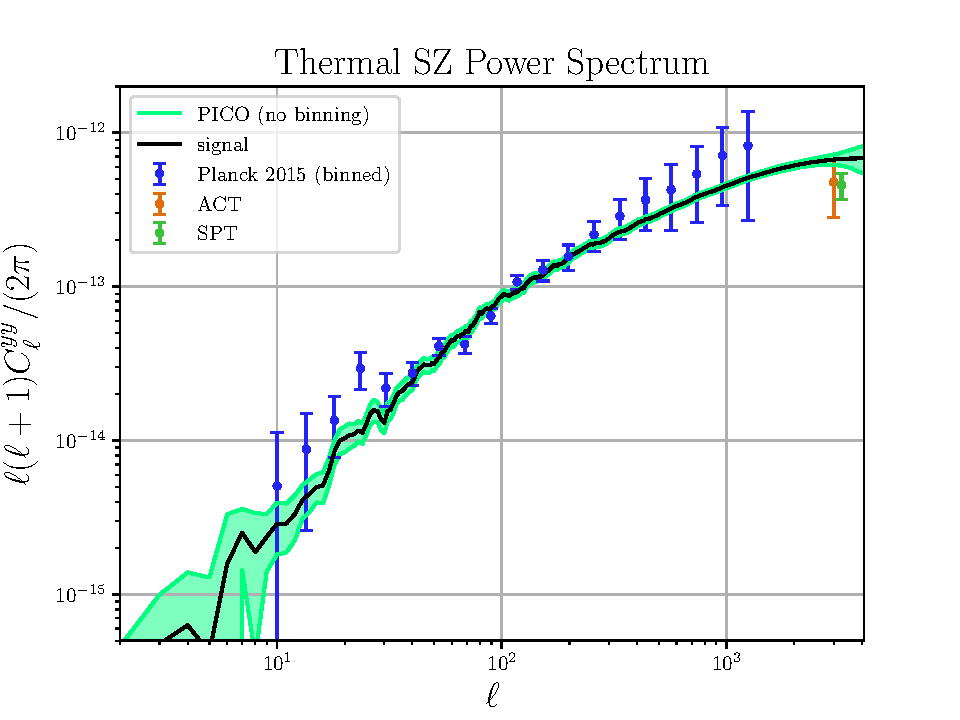
\includegraphics[width=0.8\textwidth]{images/PICO_tSZ_PS_plot.pdf}
\caption{\label{fig:PICO_tSZ_PS} Constraints on the tSZ power spectrum from PICO and current data.  The black curve shows the simulated tSZ power spectrum signal.  The light green shaded region shows the error bars for PICO at each multipole, i.e., with no binning, as determined from NILC analysis of full-sky simulations.  The blue points show the current constraints from Planck, which have been averaged into broad multipole bins.  The orange and dark green points show the constraints from ACT and SPT, respectively, at a single multipole of $\ell=3000$.  The overall PICO $S/N = 1270$, nearly two orders of magnitude larger than current measurements.}
\end{figure}

\item Cross-correlations: forecast S/N with LSST, Euclid, DESI
\end{itemize}
\item Kinematic SZ Effect
\begin{itemize}
\item Cross-correlations: forecast S/N with LSST, Euclid, DESI
\item Constraints on ICM models: figure with gas pressure and density profile plots, error bars
\item Late-time kSZ power spectrum?
\end{itemize}
\end{itemize}


\end{document}

%\begin{figure}[!htb]
%\centering
%
\includegraphics[width=4cm]{images/example}
%\caption{example}
%\label{fig:im_3}
%\end{figure}
